\documentclass{standalone}

\usepackage{tikz}
\usetikzlibrary{arrows.meta}

\begin{document}
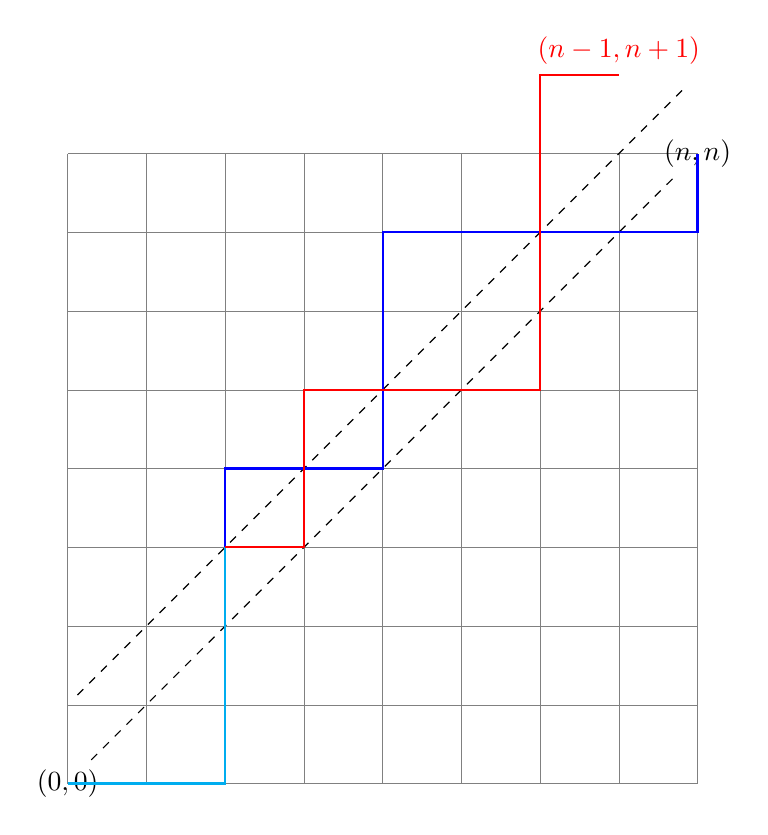
\begin{tikzpicture}
  \draw[help lines] (0,0) grid (8,8);

  \node (00) [] {$(0,0)$};
  \node (01) [] at (0,1) {};
  \node (nn) [] at (8,8) {$(n,n)$};
  \node (nn1) [] at (8,9) {};

  \draw [dashed] (00) to (nn);
  \draw [dashed] (01) to (nn1);

  \draw[thick, cyan] (0,0) -- (1,0) -- (2,0) --
	(2,1) -- (2,2) -- (2,3);
  \draw[thick, blue] (2,3) -- (2,4) --
	(3,4) -- (4,4) --
	(4,5) -- (4,6) -- (4,7) --
	(5,7) -- (6,7) -- (7,7) -- (8,7) --
	(8,8);

  \draw[thick, red] 
	(2,3) -- (3,3) --
	(3,4) -- (3,5) --
	(4,5) -- (5,5) -- (6,5) --
	(6,6) -- (6,7) -- (6,8) -- (6,9) --
	(7,9) node[above] () {$(n-1, n+1)$};
\end{tikzpicture}
\end{document}